\documentclass[12pt]{article}
\usepackage{fullpage,enumitem,amsmath,amssymb,graphicx}

\begin{document}

\begin{center}
{\Large CS221 Fall 2018 Homework [car]}

\begin{tabular}{rl}
SUNet ID: & prabhjot \\
Name: & Prabhjot Singh Rai
\end{tabular}
\end{center}

By turning in this assignment, I agree by the Stanford honor code and declare
that all of this is my own work.

\section*{Problem 1}

\begin{enumerate}[label=(\alph*)]
  \item 
  \textbf{Step 1: Remove variables that are not ancestors} \\
  \textbf{Step 2: Converting to factor graph} \\
  Step 1 and step 2 are shown in diagram below:
  \begin{center}
  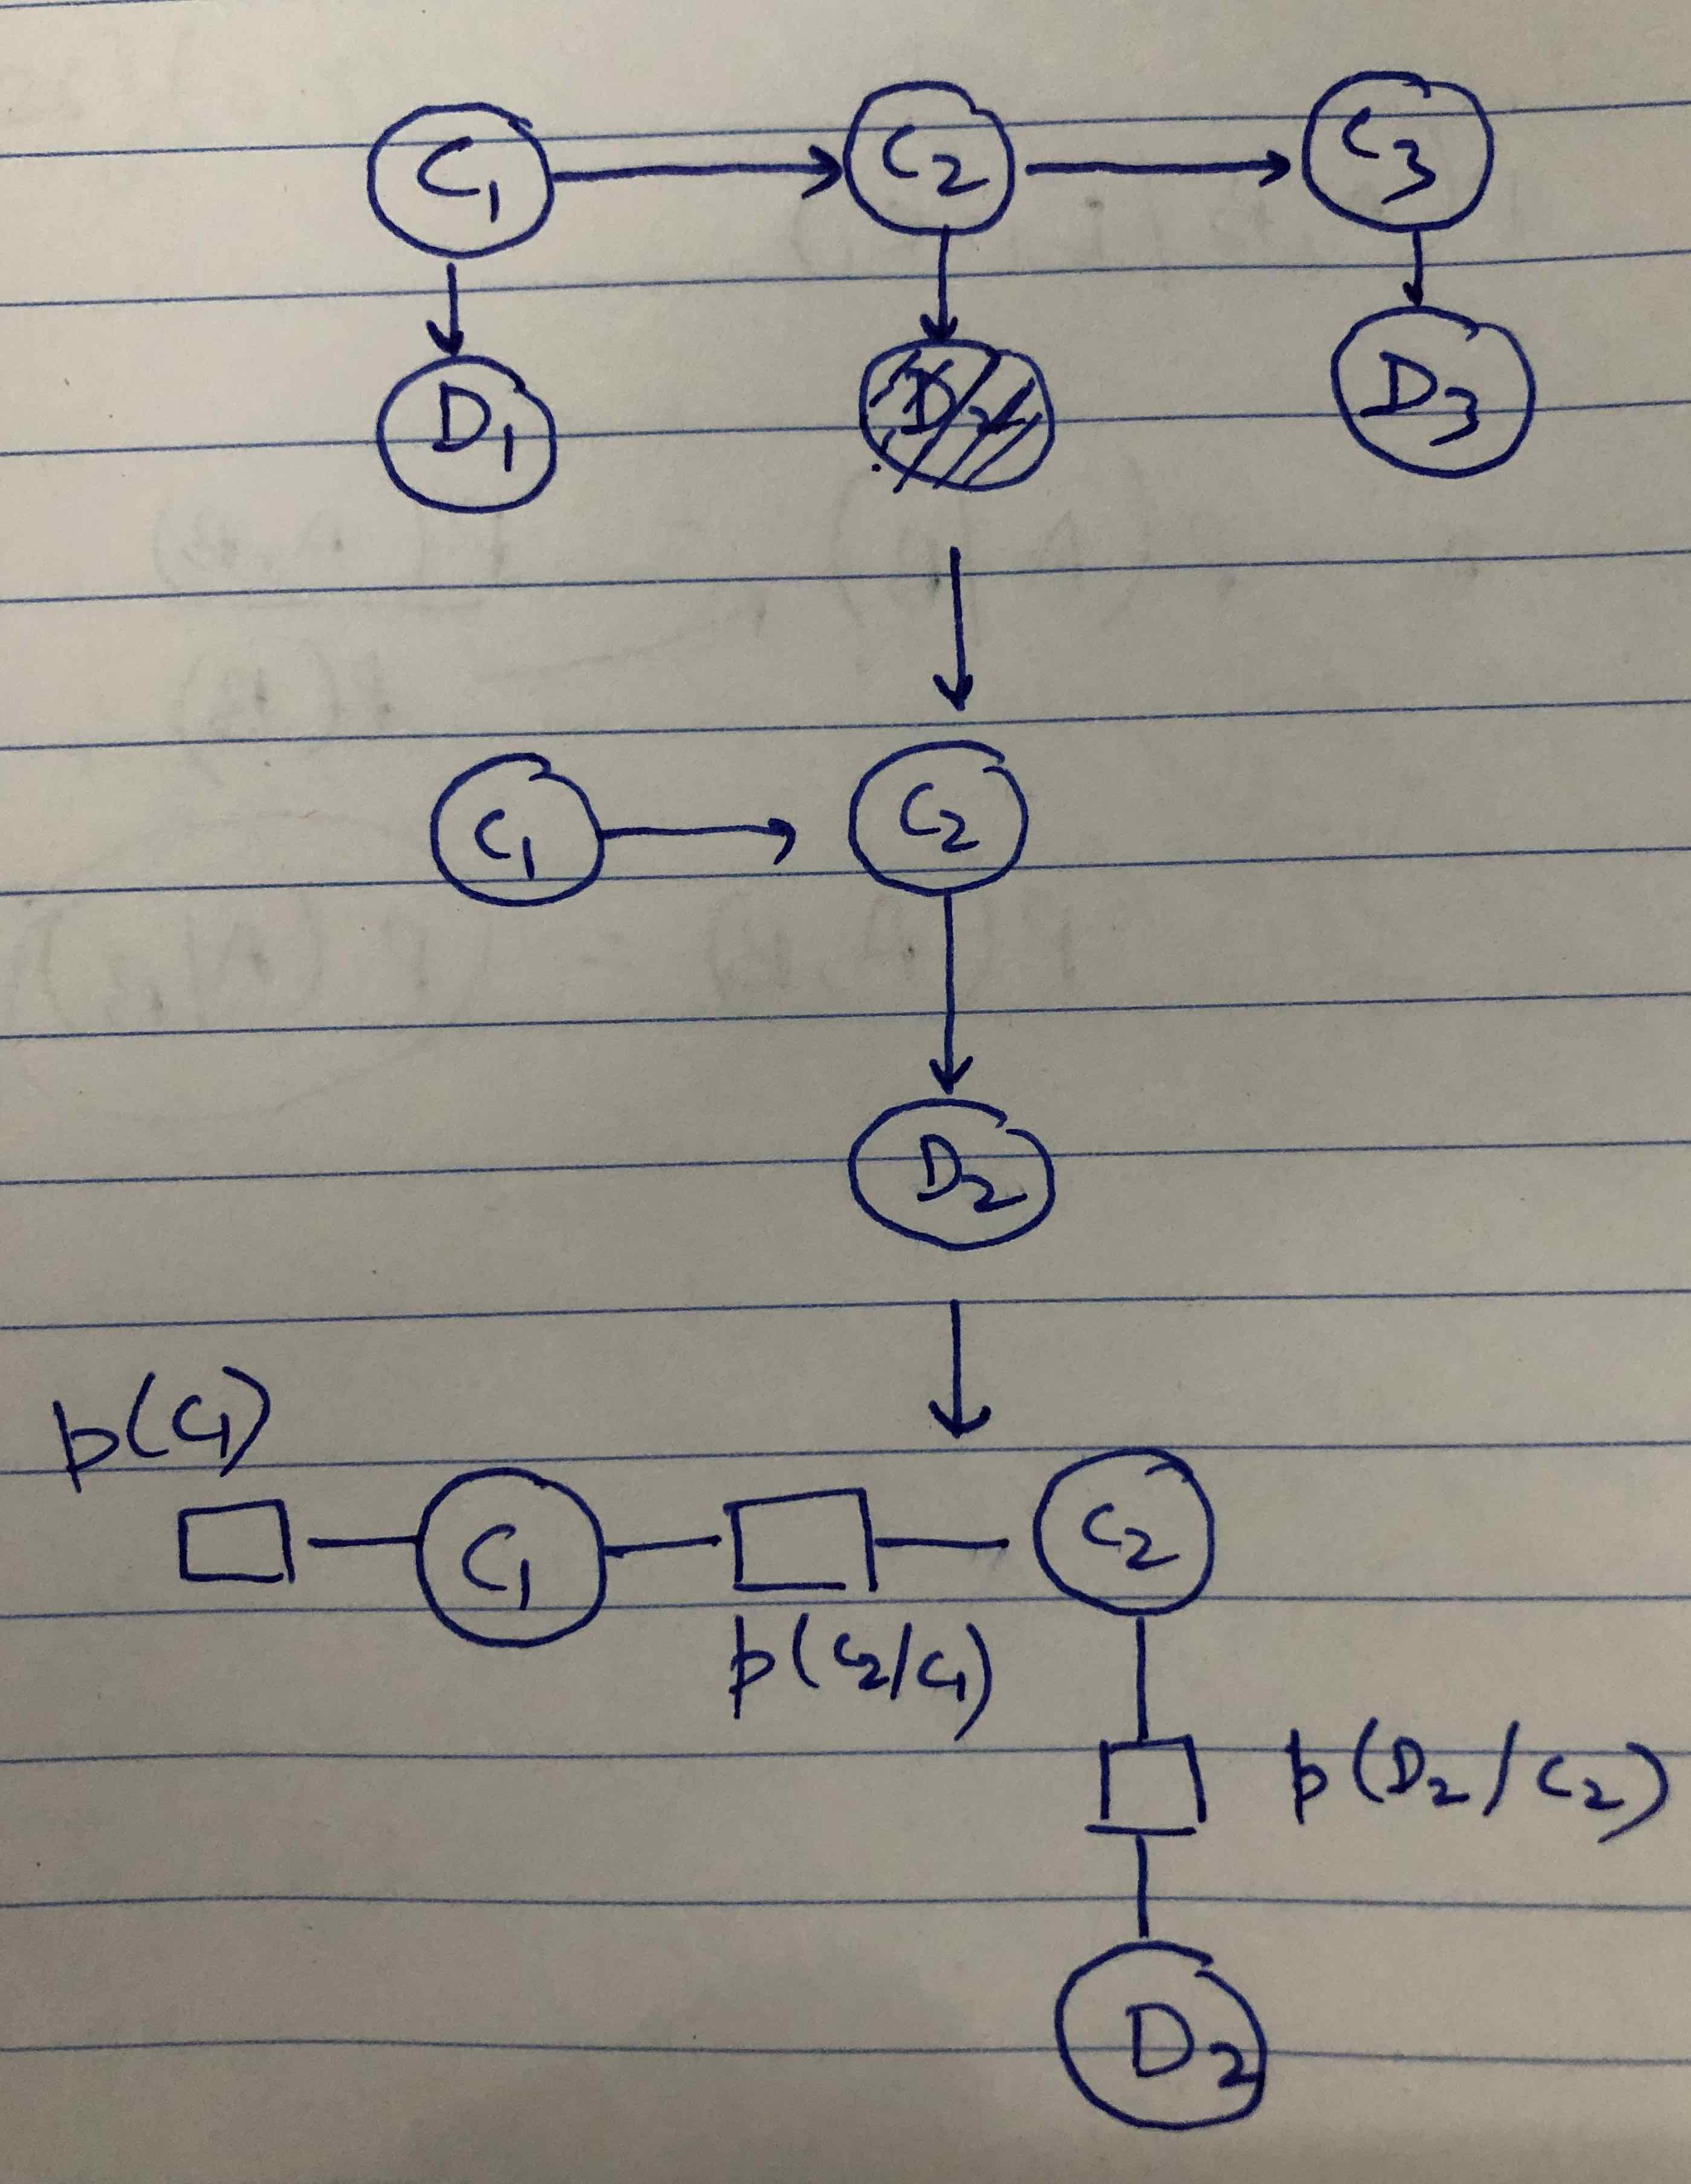
\includegraphics[scale=0.1]{IMG_2276}
  \end{center}
  \textbf{Step3: Conditioning on $D_2 = 0$} \\
  \begin{center}
  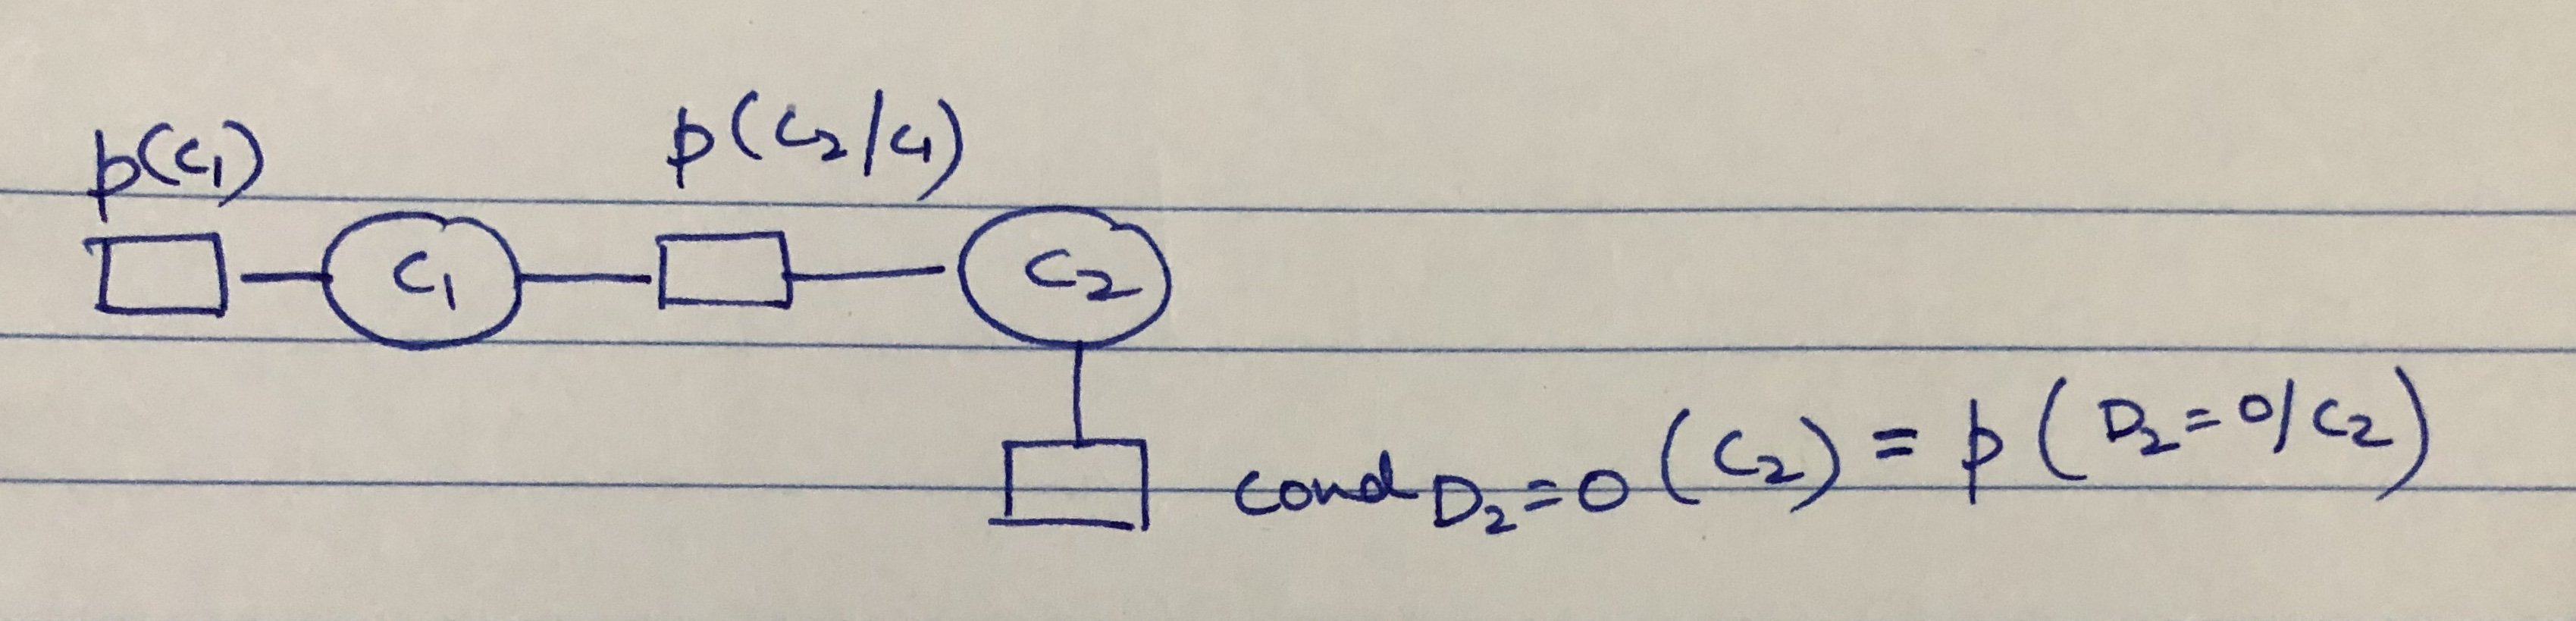
\includegraphics[scale=0.1]{IMG_2278.jpg}
  \end{center}
  Condition variable $D_2$ on value $D_2 = 0$, replacing it with a factor cond$_{D_2 = 0}(C_2)$, we get
  \begin{center}
  \begin{tabular}{ll}
  cond$_{D_2 = 0}(C_2)$ & $C_2$  \\
  $1-\eta$            & 0       \\
  $\eta$               & 1       \\
  \end{tabular} \newline \\
  \end{center}
  \textbf{Step4: Eliminate $C_1$} \\
  \begin{center}
  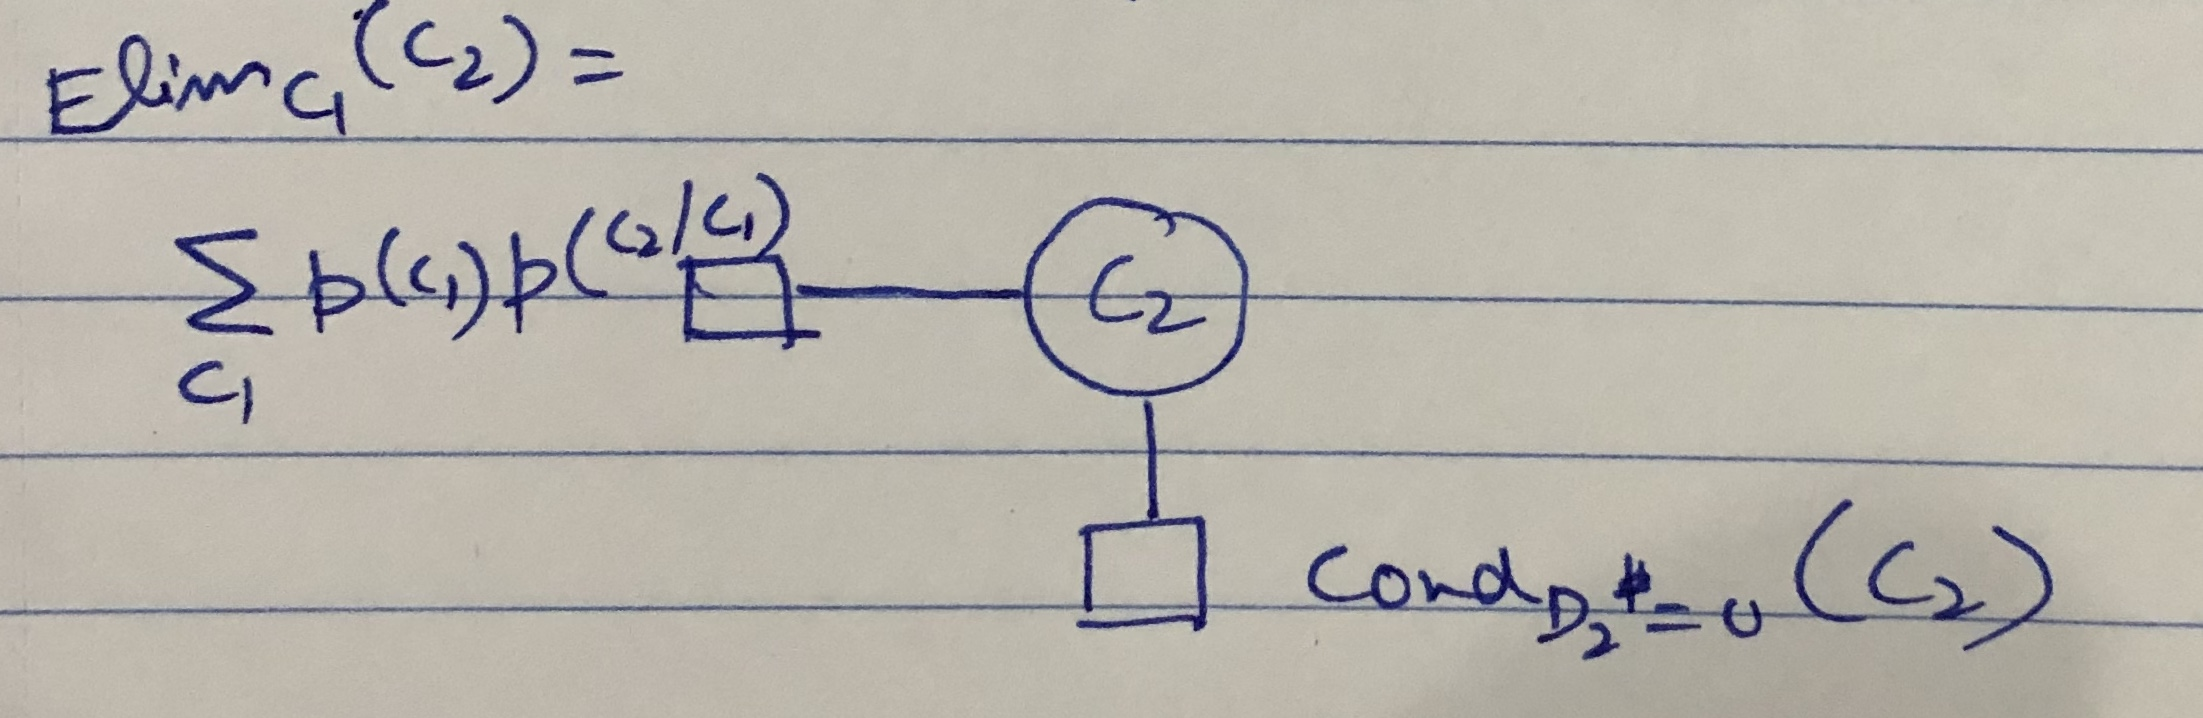
\includegraphics[scale=0.1]{IMG_2277.jpg}
  \end{center}
  \begin{align*}
	elim_{C_1}(C_2) &= \sum_{C_1} p(C_1) p(C_2/C_1) \\
	&= 0.5 \sum_{C_1} p(C_2/C_1)
  \end{align*}
  This is given from the below table:
  \begin{center}
  \begin{tabular}{ll}
  elim$_{C_1}(C_2)$ & $C_2$  \\
  $0.5(1-\epsilon + \epsilon) = 0.5$            & 0       \\
  $0.5(\epsilon + 1-\epsilon) = 0.5$               & 1       \\
  \end{tabular} \newline \\
  \end{center}
  Therefore, now that we know elim$_{C_1}(C_2)$ and cond$_{D_2 = 0} (C_2)$,
  \begin{align*}
  p(C_2/ D_2 = 0) &= \text{elim}_{C_1}(C_2) * \text{cond}_{D_2 = 0} (C_2)
  \end{align*}
  \begin{center}
  \begin{tabular}{ll}
  $p(C_2/ D_2 = 0)$ & $C_2$  \\
  $0.5 (1-\eta)$            & 0       \\
  $0.5 \eta$               & 1       \\
  \end{tabular} \newline \\
  \end{center}
  Hence, the given query,
  \begin{align*}
  p(C_2 = 1/ D_2 = 0) &= \frac{0.5 \eta}{0.5 \eta + 0.5 (1-\eta)} \\
  &= \eta
  \end{align*}
  \item 
  \textbf{Step1: Remove variables that are not ancestors} \\
  \textbf{Step2: Converting to factor graph} \\
  \textbf{Step3: Conditioning on $D_3 = 1$} \\
  Conditioning on variable $D_3$, and replacing it with a factor cond$_{D_3 = 1}(C_3)$, we get
  \begin{center}
  \begin{tabular}{ll}
  cond$_{D_3 = 1}(C_3)$ & $C_3$  \\
  $\eta$            & 0       \\
  $1-\eta$               & 1       \\
  \end{tabular} \newline \\
  \end{center}
  \textbf{Step4: Eliminating $C_3$} \\
  Defining function elim$_{C_3}(C_2)$ in order to eliminate node $C_3$ as
  \begin{align*}
  \text{elim}_{C_3}(C_2) = \sum_{C_3} \text{cond}_{D_3 = 1}(C_3) p(C_3/C_2)
  \end{align*}
  The probability distribution $p(C_3/C_2)$ is given by:
  \begin{center}
  \begin{tabular}{lll}
  C2 & C3 & p(C3/C2)    \\
  0  & 0  & $1 - \epsilon$  \\
  0  & 1  & $\epsilon$      \\
  1  & 0  & $\epsilon$      \\
  1  & 1  & $1 - \epsilon$
  \end{tabular}
  \end{center}
  The probability distribution cond$_{D_3 = 1}(C_3)$ is defined in Step 3.
  
  Combining both and substituting in equation 1, and doing summation over values of $C_3$, we will have probability distribution of elim$_{C_3}(C_2)$ is given by:
  \begin{center}
  \begin{tabular}{ll}
  $C_2$ & elim$_{C_3}(C_2)$                               \\
  0  & $(1 - \epsilon) \eta + \epsilon (1- \eta)$   \\
  1  & $\epsilon \eta + (1- \eta) (1 - \epsilon)$ 
  \end{tabular}
  \end{center}
  \textbf{Step5: Combining all factors of $C_2$} \\
  The other distribution which depends on is $p(D_2 = 1 / C_2)$, which can be conditioned as cond$_{D_2 = 0}(C_2)$, given by:
  \begin{center}
  \begin{tabular}{ll}
  $C_2$ & cond$_{D_2 = 0}(C_2)$                               \\
  0  & $1 - \eta$   \\
  1  & $\eta$ 
  \end{tabular}
  \end{center}
  Multiplying elim$_{C_3}(C_2)$ and cond$_{D_2 = 0}(C_2)$: \\ \\
  \begin{tabular}{ll}
  $C_2$ & elim$_{C_3}(C_2)$                               \\
  0  & $((1 - \epsilon) \eta + \eta (1- \epsilon)) (1 - \eta)$   \\
  1  & $(\epsilon \eta + (1- \eta) (1 - \epsilon)) \eta$ 
  \end{tabular} \newline \\
  Therefore, 
  \begin{align*}
  P(C_2 = 1/D_2 = 0, D_3 = 1) = \frac{(\epsilon \eta + (1- \eta) (1 - \epsilon)) \eta}{(\epsilon \eta + (1- \eta) (1 - \epsilon)) \eta + ((1 - \epsilon) \eta + \epsilon (1- \eta)) (1 - \eta)}
  \end{align*}
  \item
  \begin{enumerate}[label=\roman*.]
  \item
  \begin{align*}
  P(C_2 = 1/D_2 = 0) &= 0.2 \\
  P(C_2 = 1/D_2 = 0, D_3 = 1) &= 0.4157
  \end{align*}
  \item
  Adding second sensor reading increased the probability from $0.2$ to $0.4157$. Since $D_3$ is equal to 1, it means we observed the location to be 1 at location 3. This would increase the probability of $C_3 = 1$ since the emission probability $p(d_t/c_t)$ favours similar values with higher probability. $C_3 = 1$ increases the probability of $C_2 = 1$, since the transition probability $p(c_t/c_{t-1})$ favours same location with higher probability.
  \item Both the probabilities would be same when the sensor reading at $D_3$ doesn't matter. This won't matter when the transition probabilities $p(c_t/c_{t-1})$ are equal meaning no matter what is the value of $c_3$ out of all the possible values, we will get constant transition probability. This would happen when $\epsilon = 1 - \epsilon$, therefore when $\epsilon = 0.5$. 
  
  \end{enumerate}
\end{enumerate}

\section*{Problem 2}

\begin{enumerate}[label=(\alph*)]
  \item (your solution)
  \item (your solution)
\end{enumerate}

\end{document}